%%% LaTeX Template: Article/Thesis/etc. with colored headings and special fonts
%%%
%%% Source: http://www.howtotex.com/

\documentclass[12pt]{article}


\usepackage{apuntes-estilo}
\usepackage{fancyhdr,lastpage}
\usepackage{color,colortbl}
%\usepackage[dvips]{graphicx}


\def\maketitle{

% Titulo 
\makeatletter
{\color{bl} \centering \huge \sc \textbf{
Formatos internos de archivos\\
Estándares Abiertos\\
%\large \vspace*{-8pt} \color{black} Una introducción a los sistemas de archivos y atributos de archivos en GNU/Linux
 \vspace*{8pt} }\par}
 \makeatother


% Autor
 \makeatletter
 {\centering \small 
 	Departamento de Ingeniería de Computadoras \\
 	Facultad de Informática - Universidad Nacional del Comahue \\
 	\vspace{20pt} }
 \makeatother

}

% Custom headers and footers
\fancyhf{} % clear all header and footer fields
\fancypagestyle{plain}{\fancyhf{}}
  	\pagestyle{fancy}
 	\lhead{\footnotesize Formatos de archivos. Estándares abiertos - Departamento de Ingeniería de Computadoras}
 	\rhead{\footnotesize \thepage\ }	% "Page 1 of 2"

\def\ti#1#2{\texttt{#1} & #2 \\ }

\begin{document}

\thispagestyle{empty}
\maketitle
\setlength{\parindent}{0pt}


\section*{Introducción}
En el documento anterior se describieron algunos conceptos básicos sobre tipos de archivos en sistemas tipo GNU/Linux. Entre otras cosas, quedó establecido que un archivo, es simplemente un flujo de bytes.  

En esta parte analizaremos el ``formato interno'' de un archivo y su relación con las aplicaciones que permiten manipularlos. Una cuestión fundamental que surge a este respecto es el de la propiedad de los datos, es decir, quién realmente los controla. 

Además, dado que vivimos en una época digital, mucha documentación en papel se está convirtiendo en documentos electrónicos. Detrás de este movimiento hay una necesidad de interoperabilidad, de compartir la información, y de que la misma permanezca fidedigna. También es crucial que esta información pueda ser accedida sin importar el tiempo que pase. Y por otro lado, surge una cuestión de libertad al momento de elegir las diferentes aplicaciones de software. Para garantizar todo esto es necesario que los formatos utilizados al crear documentos sean independientes del proveedor y la única forma de garantizar esto es usando estándares abiertos. 

\section*{Formato interno de los archivos}

En los sistemas tipo GNU/Linux, dado que un archivo es solo una secuencia de bytes, no hay diferencia a la hora de clasificar los archivos por su contenido. Para el núcleo todos son iguales, solo son un flujo de bytes. 

Sin embargo, es diferente cómo tratan las aplicaciones a los archivos. Estás sí se encargan de verificar la naturaleza de los archivos a procesar y obrar en consecuencia al contenido de los mismos. Entonces, las aplicaciones son las que interpretan el contenido de un archivo.

Cada vez que utilizamos un archivo, los datos deben ser codificados de alguna manera para convertirlos en un flujo de bytes. Luego, cuando una aplicación debe mostrar el contenido del archivo a un usuario, deberá decodificarlo para mostrar el contenido de la manera correcta.

\begin{figure}[h]
\centering
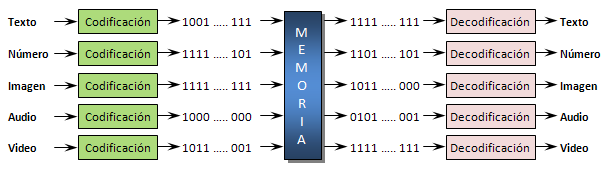
\includegraphics[width=0.8\textwidth]{patrones_bits.png}
\renewcommand{\figurename}{Fig.}
\caption{Codificación y Decodificación de bits\footnotemark}
\label{contexto:figura}
\end{figure}
\footnotetext{Forouzan - Introducción a las Ciencias Computacionales}

Definimos entonces, como formato de un archivo a la forma particular con la que se codifica la información en un archivo para que luego una aplicación pueda interpretarlo. Para los diferentes tipos de información existen distintos tipos de formatos, por ejemplo, formatos de texto, formatos de gráficos, formatos de audio, etc. Y muchas veces vamos a encontrar que en cada tipo de formato pueden existir varios formatos diferentes. Por ejemplo, este es el caso para los documentos de un procesador de texto.

Se han usado representaciones muy simples en donde por ejemplo, cierto valor numérico representa un caracter específico. Y aunque con el correr de los años, la complejidad de las representaciones ha ido aumentando, hay ciertas cuestiones que se han ido manteniendo. Dos de ellas, muy relacionadas con el objetivo de esta materia son la elección de la codificación y quién o qué aplicaciones la interpretan. 

Por un lado, con respecto a la codificación, podemos decir que la elección de la misma es arbitraria. Entonces, por ejemplo, puede ocurrir que un mismo número represente distintas letras dependiendo del código que se utilice. 

Por otro lado, una vez que el dato fue codificado en cierto formato, puede ocurrir que solo pueda ser leído por el software que implementa ese formato. Entonces al momento de utilizar un software distinto puede que el dato que obtengamos se haya corrompido o que se pierda el formato aplicado, algo muy común en el software de procesamiento de texto. Teniendo en cuenta esto, surgen los conceptos de Formato Libre y Formato Privativo.

\section*{Formato Libre vs Formato Privativo}

Al hablar de formato, nos encontramos con dos grupos generales: el privativo, y el abierto o libre. El formato privativo es aquel que está protegido por una patente o derechos de autor y por ello impone ciertas restricciones. La especificación del mismo no es pública, sino que es definida y controlada por privados. Por lo tanto, no puede ser implementado por cualquiera que desee hacerlo. Además, para su uso requiere el pago de una licencia.

Es muy común, recibir un documento y no poder leerlo por no poseer la aplicación que manipula el formato del mismo. Y al intentar obtener la aplicación nos encontramos con la situación de que debemos pagar una licencia para usarlo. Este tipo de incompatibilidad justamente se debe a que el formato utilizado es privativo. 

Por otro lado, el formato libre es una especificación definida bajo una licencia libre y por ello puede ser implementado por cualquiera sin restricciones legales. Tampoco, tiene restricciones económicas para su uso. Generalmente, es patrocinado y publicado por organizaciones de estándares abiertos. Este tipo de formato es un subconjunto de los estándares abiertos, los cuales presentaremos luego.

También existen varios formatos, que aunque algunos los consideran “híbridos”, para otros son privativos. En estos formatos, las especificaciones son públicas, pero ciertos usos, por ejemplo comercial, del software que lo manipule, puede requerir (según el país y la validez de las patentes) del pago de una licencia. Este es el caso del formato de archivos mp3, en donde podemos encontrar implementaciones libres que lo manipulan (por ejemplo LAME\footnote{http://es.wikipedia.org/wiki/LAME_(codificador)}). Sin embargo, en Argentina, no podríamos vender nuestro propio reproductor de mp3 sin pagar la licencia apropiada\footnote{http://mp3licensing.com/help/developers.html\#51}, aún cuando en él utilicemos una implementación libre. 

Una de las cuestiones que surge acerca del uso de formatos propietarios, es la de la propiedad\footnote{http://es.wikipedia.org/wiki/Formato\_propietario}. Aunque el usuario posea la información, si esta es almacenada en un formato en el que el proveedor impone restricciones, no podrá extraerla si no utiliza el software controlado por dicho proveedor. Por lo cual finalmente el control de la información en realidad no lo tiene el usuario. Además, si el proveedor lanza al mercado nuevas versiones del software o decide dejar de fabricar el producto, toda la información del usuario quedará ligada a un formato obsoleto.  

Por otro lado, el tener que utilizar un único software para manipular los datos almacenados, favorece el monopolio del mercado por parte del proveedor. Cualquier persona que necesite leer la información, debe tener el software correspondiente. Esto por supuesto, no permite que se comparta libremente la información. Por ello, es un problema para las personas, empresas y gobiernos que utilizan el formato privativo.

En oposición a todo esto, los formatos abiertos garantizan el acceso a largo plazo a los datos almacenados, evitando la incertidumbre del usuario con respecto a los derechos legales del uso de la tecnología de acceso, a la disponibilidad de la misma, o a la especificación técnica del formato de almacenamiento de los datos\footnote{http://es.wikipedia.org/wiki/Formato\_abierto}. Además un formato libre puede ser soportado por un número mayor de aplicaciones, incluso por aquellas privativas, lo cual permite mayor interoperabilidad.  

\section*{Estándares abiertos}

Dada la necesidad de que diferentes programas de software puedan intercambiar datos y de que los usuarios no estén sujetos a determinados formatos de documentos y con ello a ciertas empresas de software, mucho se ha empezado a hablar de los Estándares Abiertos. 

Existen varias definiciones de lo que es un Estándar abierto, y no hay una que haya sido aceptada universalmente. Una de ellas es la que usa la FSFE (Free Software Foundation Europe), que se basa en el Framework de Interoperabilidad Europeo. Entonces un Estándar Abierto\footnote{http://fsfe.org/activities/os/def.es.html} hace referencia a un formato o protocolo que: 
\begin{itemize}
\item esté sujeto a una evaluación pública completa, se pueda usar sin restricciones y esté disponible por igual para todas las partes;
\item no necesite ningún componente o extensión adicional que tenga dependencias con formatos o protocolos que no cumplan la definición de un Estándar Abierto;
\item esté libre de cláusulas legales o técnicas que limiten su utilización por cualquier parte o en cualquier modelo de negocio;
\item esté gestionado y pueda ser desarrollado independientemente por cualquier compañía en un proceso abierto a la participación equitativa por parte de competidores y terceras partes;
\item esté disponible en varias implementaciones completas por compañías en competencia, o como una implementación completa disponible para todas las partes.
\end{itemize}

Tomando como base esta definición, vemos que si se utiliza un Estándar Abierto es posible intercambiar la información, independientemente del software que se use. Además, la independencia del software asegura que aunque pasen los años e incluso el software que se usó para generarla no exista, la información va a poder ser accedida por cualquier otro software que cumpla con el estándar. Entonces, una especificación pública y abierta garantiza la preservación, durabilidad, integridad y reusabilidad de la información sin restricciones\footnote{http://ftacademy.org/standards}. 

Por otro lado, los Estándares Abiertos favorecen la competencia en el mercado y promueven la innovación. Un ejemplo de esto es Internet mismo, en donde la propia naturaleza de los estándares estabiliza una plataforma sobre la cual los competidores pueden crear soluciones innovadoras e interoperables. 
 
\section*{Uso de Estándares Abiertos en el Estado Público}

El Estado Público como administrador de los recursos de todos los ciudadanos debe usar formatos libres por varias razones:
\begin{itemize}
\item Para asegurar el acceso a la información sin importar el tiempo que pase, incluso aunque el software utilizado para producirla sea obsoleto.

\item Para asegurar el acceso libre de todos los ciudadanos a la información pública, evitando que estos tengan que usar y/o comprar el software utilizado para producir la información. Así el Estado evita actuar como promotor del producto del fabricante.

\item Para poder compartir datos entre las administraciones nacionales, provinciales y municipales. Esto asegura la interoperabilidad.

\item Para ser independientes del proveedor. Con el software privativo y la utilización de formatos cerrados no hay libertad de contratación. Se produce una dependencia tecnológica en la que el proveedor está en condiciones de dictar unilateralmente términos, plazos y precios, ya que si no se aceptan sus condiciones, se puede perder la información así como quedar aislado del universo informático. Mediante la utilización de formatos abiertos se permite a diversos proveedores desarrollar software destinado al manejo de la información almacenada. Por otra parte, se estimula la competencia y el desarrollo de software a nivel nacional.

\item Para tener la posibilidad de auditar el funcionamiento de un software que use un formato libre. En el caso en que utilice un formato cerrado, debe confiar en su funcionamiento y en que se mantenga privada la información que mantiene.

\item Para asegurar la privacidad de la información. El uso de formatos cerrados crea un riesgo de privacidad de quien elabora el documento en el que no hay seguridad de que las partes supuestamente borradas hayan sido efectivamente removidas y no solo marcadas como borradas y por lo tanto permanezcan en el documento. 
\end{itemize}

A este respecto, son varios los países que han empezado a utilizar formatos abiertos:
\begin{itemize}
\item En los Estados Unidos, Massachusetts se convirtió en el primer Estado en legislar específicamente respecto a los formatos abiertos por su importancia para los archivos públicos\footnote{http://www.cio.com/article/2438324/open-source-tools/massachusetts-adopts-open-documents-format-compromise.html
\\http://xml.coverpages.org/ni2005-03-25-a.html}. El formato elegido inicialmente fue OpenDocument. Así mismo se indicó que a partir del 2007 solo se utilizaría software de aquellas empresas que soportaran formatos abiertos.
\item En Uruguay, el 8 de enero de 2014 fue publicada la Ley Nº 19179 ``Software libre y formatos abiertos en el estado'', la cual obliga a cualquier organismo dependiente o ligado al Estado a ``distribuir toda información en al menos un formato abierto, estándar y libre.'' Además ``Todo pedido de información deberá ser aceptado en al menos un formato abierto y estándar''\footnote{http://www.parlamento.gub.uy/leyes/AccesoTextoLey.asp?Ley=19179}.
\item En Bélgica, el 23 de junio de 2006, el Gobierno Federal decidió que el formato OpenDocument fuese obligatorio a partir de septiembre de 2008. Además Bélgica es el primer estado en el mundo que prohíbe de facto el uso de formatos propietarios.
\item En Holanda, en noviembre de 2007 se estableció, por ley, una fecha límite para que las administraciones públicas adopten estándares abiertos.
\item En España la ley 11/2007 de ``Acceso Electrónico de los ciudadanos a los Servicios Públicos'' establece que las Administraciones Públicas deben utilizar estándares abiertos y, en forma complementaria, estándares que sean de uso generalizado por parte de los ciudadanos. Esta norma es aplicada junto con el Real Decreto 4/2010\footnote{http://www.boe.es/boe/dias/2010/01/29/pdfs/BOE-A-2010-1331.pdf} por el que se regula el Esquema Nacional de Interoperabilidad en el ámbito de la Administración Electrónica y la Norma Técnica de Interoperabilidad de Catálogo de estándares\footnote{https://www.boe.es/diario\_boe/txt.php?id=BOE-A-2012-13501}.
\item En el Reino Unido, recientemente se anunció el uso de formatos abierto para todas las oficinas de gobierno\footnote{https://www.gov.uk/government/news/open-document-formats-selected-to-meet-user-needs}.
\item En Argentina también se ha promovido el uso de estándares abiertos. Los diputados Eduardo Macaluse, Claudio Lozano, Ricardo Cuccovillo y Nélida Beluos firmaron el proyecto que lleva el número 5914-D-2010\footnote{http://www1.hcdn.gov.ar/proyxml/expediente.asp?fundamentos=si\&numexp=2161-D-2013} para promover el uso obligatorio de Estándares Abiertos en los sistemas de información del Estado, con el objetivo de garantizar la interoperabilidad en los sistemas de información utilizados en todas sus dependencias entre sí y con los particulares.
\end{itemize}

También es digno de mención un evento que se celebra el último miércoles de marzo de cada año. Este es el ``\textbf{Día de los Documentos Libres}''. Ese día, las personas que creen en el acceso justo a la tecnología de las comunicaciones, enseñan, actúan y se manifiestan para concientizar a otros sobre los formatos y estándares abiertos.\footnote{http://documentfreedom.org/index.es.html}


\section*{Migracion de documentos a formatos abiertos}

Aunque el uso de formatos abiertos supone muchas ventajas, en muchas organizaciones la información ya está almacenada en formatos cerrados. Por lo tanto, al decidir comenzar a usar formatos abiertos, surge la necesidad de migrar de un formato a otro. Y esto no siempre es sencillo. 
Algunos problemas que pueden presentarse son:
\begin{itemize}
\item Interoperabilidad de documentos: el formato cerrado por definición es un formato protegido por una patente o derechos de autor. Por lo tanto no siempre se logra conocer toda la especificación del mismo. Entonces, una técnica que se utiliza es la de ingeniería inversa\footnote{http://es.wikipedia.org/wiki/Ingeniería\_inversa} con el objetivo de descubrir cómo funciona un determinado formato, para luego generar código propio que permita manipularlo. Sin embargo, no siempre es posible llegar a conocer la especificación completa, por lo cual al migrar de un formato a otro, no es posible obtener la información de la misma manera que se encontraba con el formato cerrado.
\item Resistencia del usuario al cambio. Muchos tienen miedo a lo desconocido y su primera reacción es negativa. Entonces es necesario instrumentar mecanismos para minimizar esta resistencia.
\end{itemize}


\section*{Licencia}
Copyright (C) 2014 Claudia Rozas, Miriam Lechner.

Se concede autorización para copiar, distribuir y/o modificar este documento
bajo los términos de la Licencia Creative Commons Atribución-CompartirDerivadasIgual 3.0 Unported. 

http://creativecommons.org/licenses/by-sa/3.0/
\end{document}

